\documentclass[12pt]{presentation}
%\documentclass[compress]{beamer}
\usetheme{default}
%\usecolortheme{whale}
\usepackage{ulem}
\usepackage{amsmath}
\usepackage{url}
\usepackage{graphicx}
\usepackage{pgf}
\usepackage{pgfplots}
\usepackage{tikz}
\usetikzlibrary{fit}					% fitting shapes to coordinates
\usetikzlibrary{backgrounds}	% drawing the background after the foreground
\usetikzlibrary{arrows,automata,calc,patterns,snakes}
\usepackage[latin1]{inputenc}
\usepackage{verbatim}
\usepackage{color, colortbl}

\newcommand{\vocab}{\mathbf{v}}
\newcommand{\dtvec}{\mathbf{t}_\Delta}
\newcommand{\ctxvec}{\mathbf{t}_\text{ctx}}
\newcommand{\dt}{\Delta_t}
\newcommand{\prerror}{Pr_{error}}
\newcommand{\fvec}{\mathbf{X}}
\newcommand{\weights}{\mathbf{w}}
\newcommand{\X}{\mathbf{X}}
\setbeamertemplate{footline}{\insertframenumber/\inserttotalframenumber}
\title{Predicting Web 2.0 Thread Updates\\Progress Update}
\author{Shawn Tan}
\AtBeginSection[]
{
	\begin{frame}{Table of Contents}
	\tableofcontents[currentsection]
	\end{frame}
}
\date{}

\begin{document}
\maketitle
\section{Introduction}

\begin{frame}{Motivation}
	\begin{itemize}
		\item Many sites with thread-based discussion features
		\item Users post product reviews, feedback
	\end{itemize}
	Obtaining such up-to-date information may be vital to companies.
\end{frame}
\section{The Dataset}
\begin{frame}{avsforum.com}
	\begin{center}
		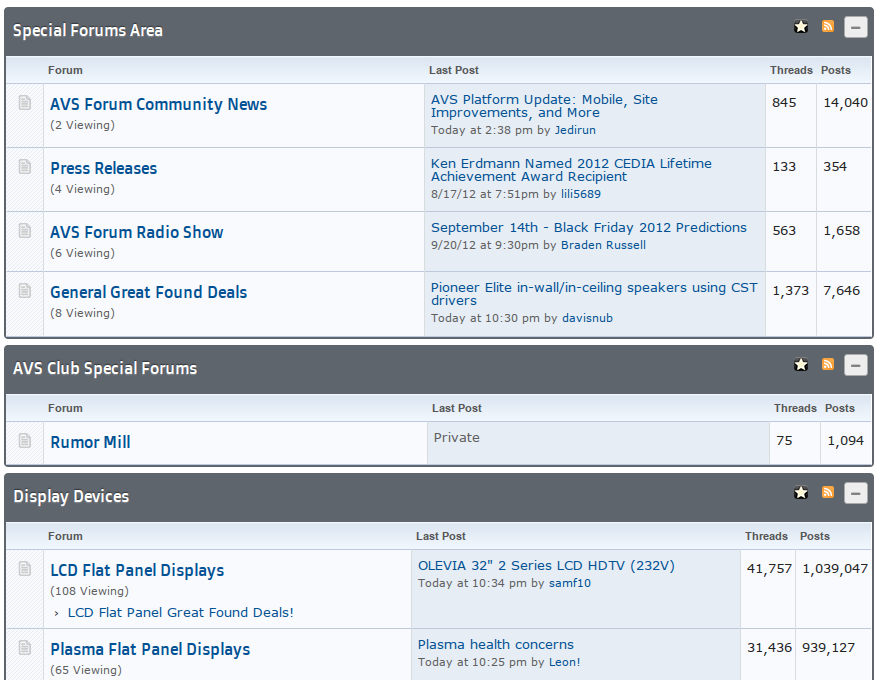
\includegraphics[scale=0.3]{screenshots/index.png}
	\end{center}
\end{frame}

\begin{frame}{User-centric threads}
	\begin{center}
		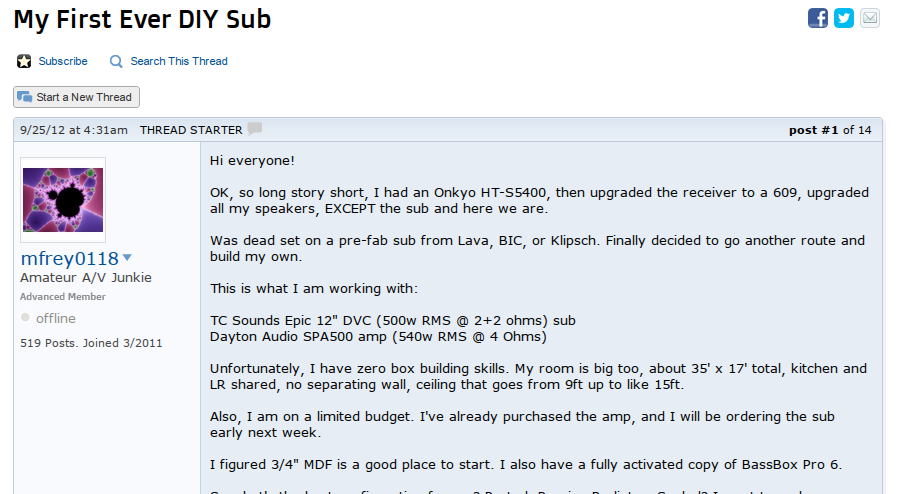
\includegraphics[scale=0.2]{screenshots/revolve_user.png}\\
			$\vdots$\\
		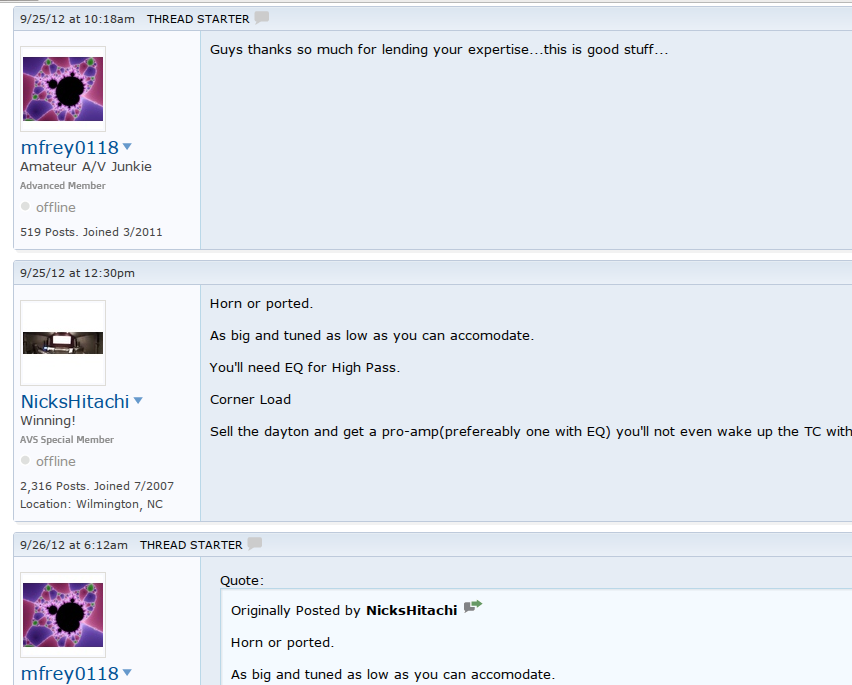
\includegraphics[scale=0.2]{screenshots/revolve_user2.png}
	\end{center}
\end{frame}


\begin{frame}{Questions}
	\begin{center}
		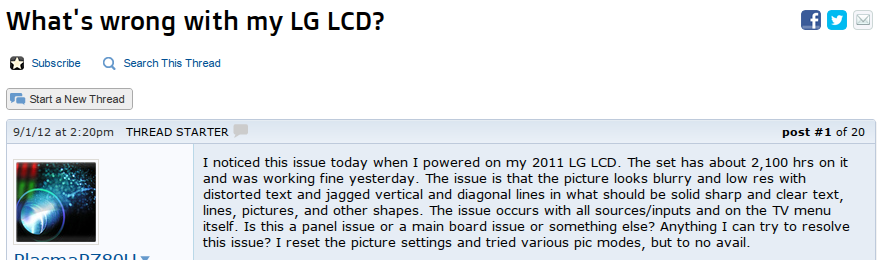
\includegraphics[scale=0.4]{screenshots/question.png}\\
			$\vdots$\\
		
\includegraphics[scale=0.4]{screenshots/question2.png}
	\end{center}
\end{frame}


\begin{frame}{Mentions}
	\begin{center}
		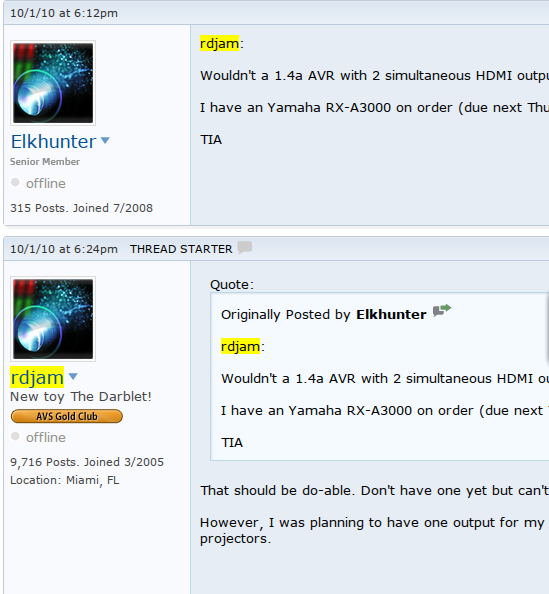
\includegraphics[scale=0.4]{screenshots/replies.png}\\
	\end{center}
\end{frame}


\section{Evaluation Methods}
\begin{frame}{Requirements}
	\begin{itemize}
		\item Balance of freshness and bandwidth usage.
		\item Penalise when using too much bandwidth (visiting the site too 
			much).
		\item Penalise when ``database" not fresh (visiting the site too 
			little).
	\end{itemize}
\end{frame}
\begin{frame}{Events}
\begin{center}
	
\tikzstyle{background}=[rectangle,
	fill=gray!10,
	inner sep=0.2cm,
	rounded corners=5mm]


\tikzstyle{post}=[circle,
	thick,
	minimum size=1.2cm,
	draw=blue!80,
	fill=blue!20]
% The measurement vector is represented by an orange circle.
\tikzstyle{visit}=[circle,
	thick,
	minimum size=1.2cm,
	draw=orange!80,
	fill=orange!25]

\begin{tikzpicture}[>=latex,text height=1.5ex,text depth=0.25ex]
    % "text height" and "text depth" are required to vertically
    % align the labels with and without indices.
  
  % The various elements are conveniently placed using a matrix:
  \matrix[column sep=0.3cm] {
    % First line: Control input
    	&
		\node (e0)					{};&
		\node (e1)	[post]			{};&
		\node (e2)	[visit]			{};&
		\node (e3)	[post]			{};&
		\node (e4)	[visit]			{};&
		\node (e5)	[post]			{};&
		\node (e6)	[visit]			{};&
		\node (e)					{};&
		&
        \\
	};
    
    % The diagram elements are now connected through arrows:

	\path[-]
		(e0) edge[thick]	(e1)
		\foreach \e in {1,2,3,4,5}{
			let \n1={int(\e+1)} in (e\e) edge[thick] (e\n1)
		}
		(e6) edge[thick]	(e)
	;

	\begin{pgfonlayer}{background}
		\node [background,fit=(e1) (e3)] {};
	\end{pgfonlayer}

\end{tikzpicture}


\begin{tikzpicture}[>=latex,text height=1.5ex,text depth=0.25ex]
    % "text height" and "text depth" are required to vertically
    % align the labels with and without indices.
  
  % The various elements are conveniently placed using a matrix:
  \matrix[column sep=0.3cm] {
    % First line: Control input
    	&
		\node (e0)					{};&
		\node (e1)	[post]			{}; &
		\node (e2)	[visit]			{}; &
		\node (e3)	[post]			{}; &
		\node (e4)	[visit]			{}; &
		\node (e5)	[post]			{}; &
		\node (e6)	[visit]			{}; &
		\node (e)					{};&
		&
        \\
	};
    
    % The diagram elements are now connected through arrows:

	\path[-]
		(e0) edge[thick]	(e1)
		\foreach \e in {1,2,3,4,5}{
			let \n1={int(\e+1)} in (e\e) edge[thick] (e\n1)
		}
		(e6) edge[thick]	(e)
	;

	\begin{pgfonlayer}{background}
		\node [background,fit=(e3) (e5)] {};
	\end{pgfonlayer}

\end{tikzpicture}

\end{center}
\end{frame}
\begin{frame}{$T$-score}
\begin{center}
	\input{t_score_diag}
\end{center}
\[
	T = \frac{1}{N} \sum_{i \in posts} \Delta_i
\]
From Yang et. al. 2009
\end{frame}
\begin{frame}{Visit/Post ratio}
	\large
	Number of visits per post, keep the $T$-score in check.
\end{frame}
\begin{frame}{$Pr_{error}$}
	\begin{center}
	
\tikzstyle{background}=[rectangle,
	fill=gray!10,
	inner sep=0.2cm,
	rounded corners=5mm]


\tikzstyle{post}=[circle,
	thick,
	minimum size=1.2cm,
	draw=blue!80,
	fill=blue!20]
% The measurement vector is represented by an orange circle.
\tikzstyle{visit}=[circle,
	thick,
	minimum size=1.2cm,
	draw=orange!80,
	fill=orange!25]

\begin{tikzpicture}[>=latex,text height=1.5ex,text depth=0.25ex]
    % "text height" and "text depth" are required to vertically
    % align the labels with and without indices.
  
  % The various elements are conveniently placed using a matrix:
  \matrix[column sep=0.4cm] {
    % First line: Control input
    	&
		\node (e0)				{$\cdots$};&
		\node (e1)	[post]			{$\rho_1$}; &
		\node (e2)	[visit]			{$\rho_2$}; &
		&&
		\node (e3)	[post]			{$\rho_5$}; &
		\node (e4)	[visit]			{$\rho_6$}; &
		&&
		\node (e)				{$\cdots$};&
		&
        \\
	};
    
    % The diagram elements are now connected through arrows:

	\path[-]
		(e0) edge[thick]	(e1)
		\foreach \e in {1,2,3}{
			let \n1={int(\e+1)} in (e\e) edge[thick] (e\n1)
		}
		(e4) edge[thick]	(e)
	;
	\begin{pgfonlayer}{background}
		\only<1>{\node [background,fit=(e1) (e3)] {};}
		\only<2>{\node [background,fit=(e2) (e4)] {};}
    \end{pgfonlayer}


\end{tikzpicture}

	\end{center}
\begin{enumerate}
	\item $Pr_{fa}$ More visits than posts, false alarm.
	\item $Pr_{miss}$ More posts than visits, miss.
\end{enumerate}
Weighted average use as error metric.
\[Pr_{error} = \alpha Pr_{fa} + (1 - \alpha) Pr_{miss}\]

Georgescul et. al. 2006
\end{frame}


\section{Initial Experiments}


\begin{frame}{Baseline}
Take the average $\Delta_t$ from training set, and use that as the revisit time.
	\begin{center}
		\begin{tabular}{ | l | c | c | c | }
			\hline
		& $Pr_{error}$		  & $T$-score			   &	Visit/Post\\
			\hline
 Average &		0.501 $\pm$ 0.001 &	1764.474 $\pm$ 267.227  &	18.117 $\pm$ 7.290 \\
			\hline
		\end{tabular}
	\end{center}

\end{frame}

\begin{frame}{Windowing}
Use features from windows of posts. Number of posts in window given by $w$.
\begin{center}
\tikzstyle{background}=[rectangle,
	fill=gray!10,
	inner sep=0.2cm,
	rounded corners=5mm]


\tikzstyle{post}=[circle,
	thick,
	minimum size=0.75cm,
	draw=blue!80,
	fill=blue!20]
% The measurement vector is represented by an orange circle.
\tikzstyle{visit}=[circle,
	thick,
	minimum size=0.75cm,
	draw=orange!80,
	fill=orange!25]

\begin{tikzpicture}[>=latex,text height=1.5ex,text depth=0.25ex]
    % "text height" and "text depth" are required to vertically
    % align the labels with and without indices.
  
  % The various elements are conveniently placed using a matrix:
  \matrix[column sep=0.3cm] {
    % First line: Control input
    	&
		\node (e0)					{};&
		\node (e1)	[post]			{}; &
		\node (e2)	[visit]			{}; &
		&&
		\node (e3)	[post]			{}; &
		\node (e4)	[post]			{}; &
		&&
		\node (e5)	[visit]			{}; &
		\node (e6)	[post]			{}; &
		\node (e7)	[visit]			{}; &
		\node (e)					{};&
		&
        \\
	};
    
    % The diagram elements are now connected through arrows:

	\path[-]
		(e0) edge[thick]	(e1)
		\foreach \e in {1,2,3,4,5,6}{
			let \n1={int(\e+1)} in (e\e) edge[thick] (e\n1)
		}
		(e7) edge[thick]	(e)
	;
	\begin{pgfonlayer}{background}
		\only<1>{\node [background,fit=(e1) (e3)] {};}
		\only<2>{\node [background,fit=(e3) (e4)] {};}
		\only<3>{\node [background,fit=(e4) (e6)] {};}
    \end{pgfonlayer}


\end{tikzpicture}

\end{center}
\end{frame}


\begin{frame}{Window-based average}
	Take the average $\Delta_t$ from \sout{training set} the previous window, and use that as the revisit time.
	\begin{center}
		\footnotesize
		\begin{tabular}{ | l | c | c | c | }
			\hline
		& $Pr_{error}$		  & $T$-score			   &	Visit/Post\\
			\hline
 $w = 1$ &	0.504 $\pm$ 0.003 &	18862.320 $\pm$ 4267.812 &	16.142 $\pm$ 7.049 \\
 $w = 5$ &	0.502 $\pm$ 0.003 &	6418.208 $\pm$ 962.716 &  	16.464 $\pm$ 7.386 \\
 $w = 10$ &	0.504 $\pm$ 0.003 &	4598.955 $\pm$ 682.458 &  	17.291 $\pm$ 7.872 \\
$w = 15$ &	0.504 $\pm$ 0.003 &	3833.605 $\pm$ 600.824 &  	18.337 $\pm$ 8.727 \\
\rowcolor{green}
$w = 20$ &	0.504 $\pm$ 0.003 &	3340.929 $\pm$ 444.908 &  	18.102 $\pm$ 8.541 \\
			\hline
		\end{tabular}
	\end{center}
	Performs worse than the simple average baseline.

\end{frame}

\begin{frame}{Support Vector Regression}
		Using only the window's $\Delta_t$ as features.
	\begin{center}
		\footnotesize
		\begin{tabular}{ | l | c | c | c | }
			\hline
		& $Pr_{error}$		  & $T$-score			   &	Visit/Post\\
			\hline
  $w=1$ &	0.498 $\pm$ 0.002 &	1576.082 $\pm$ 253.300 &  	18.267 $\pm$ 7.290 \\
  $w=5$ &	0.498 $\pm$ 0.002 &	1541.595 $\pm$ 232.272 &  	17.907 $\pm$ 7.508 \\
 $w=10$ &	0.499 $\pm$ 0.002 &	1488.688 $\pm$ 196.648 &  	18.371 $\pm$ 7.947 \\
\rowcolor{green}
 $w=15$ &	0.500 $\pm$ 0.002 &	1443.138 $\pm$ 183.408 &  	19.234 $\pm$ 8.805 \\
 $w=20$ &	0.499 $\pm$ 0.001 &	1584.171 $\pm$ 227.209 &  	18.880 $\pm$ 8.602 	\\
			\hline
		\end{tabular}
	\end{center}
	Performs better than baseline, but, what happens if we use content?
\end{frame}

\begin{frame}{Content-based features}
	Count of individual tokens used:
	\begin{enumerate}
		\item Text is stemmed, stopwords removed
		\item Occurences of usernames are replaced with `\#USER\#'
		\item Occurences of tokens with mixtures of alphabets and numbers are 
			replaced with `\#MODEL\#'
		\item Univariate regression tests used to select features
	\end{enumerate}
\end{frame}
\begin{frame}{Time-context}
	\begin{enumerate}
		\item Hour of the day
		\item Day of the week
	\end{enumerate}
	Represented as bit vectors
\end{frame}

\begin{frame}{Content features only}
	Using only the content features (stemmed word frequency counts).
	\begin{center}
		\footnotesize
		\begin{tabular}{ | l | c | c | c | }
			\hline
		& $Pr_{error}$		  & $T$-score			   &	Visit/Post\\
			\hline
        $w=1$ &		0.496 $\pm$ 0.002 &	1649.606 $\pm$ 262.578  &	18.255 $\pm$ 7.292 \\
        $w=5$ &		0.495 $\pm$ 0.001 &	1596.220 $\pm$ 234.643  &	17.859 $\pm$ 7.508 \\
       $w=10$ &		0.498 $\pm$ 0.001 &	1554.391 $\pm$ 196.343 &  	18.341 $\pm$ 7.949 \\
\rowcolor{green}
       $w=15$ &		0.497 $\pm$ 0.001 &	1500.391 $\pm$ 185.857 &  	19.197 $\pm$ 8.808 \\
       $w=20$ &		0.494 $\pm$ 0.002 &	1653.162 $\pm$ 230.106 &  	18.859 $\pm$ 8.606 \\
			\hline
		\end{tabular}
	\end{center}
	Worse than the time difference approach, would using both sets of features help?
\end{frame}


\begin{frame}{Content features $+ \Delta_\mathbf{t} + $ time-context}
	\begin{center}
		\footnotesize
		\begin{tabular}{ | l | c | c | c | }
			\hline
		& $Pr_{error}$		  & $T$-score			   &	Visit/Post\\
			\hline
 $w=1$ &	0.498 $\pm$ 0.002 &	1537.992 $\pm$ 251.250 &  	18.272 $\pm$ 7.291 \\
 $w=5$ &	0.498 $\pm$ 0.002 &	1541.587 $\pm$ 232.271 &  	17.907 $\pm$ 7.508 \\
$w=10$ &	0.499 $\pm$ 0.002 &	1488.669 $\pm$ 196.646 &  	18.371 $\pm$ 7.947 \\
\rowcolor{green}
$w=15$ &	0.500 $\pm$ 0.002 &	1443.130 $\pm$ 183.407 &  	19.234 $\pm$ 8.805 \\
$w=20$ &	0.499 $\pm$ 0.001 &	1584.171 $\pm$ 227.209 &  	18.880 $\pm$ 8.602 \\
			\hline
		\end{tabular}
	\end{center}
	Improved performance by an hour on average, still nothing significant.
\end{frame}


\section{Different Approaches}
\begin{frame}{Discounted Sum}
	Discounted sum of feature vectors from previous windows.
\[
	\fvec_t = \vocab_t + \gamma \fvec_{t-1}
\]
Where $0 > \gamma > 1$. Here we use only the word count as before.
	\begin{center}
		\footnotesize
		\begin{tabular}{ | l | c | c | c | }
			\hline
		& $Pr_{error}$		  & $T$-score			   &	Visit/Post\\
			\hline
 $\alpha=0.1$ &	0.500 $\pm$ 0.002 &	1443.129 $\pm$ 183.407 &	19.234 $\pm$ 8.805 \\
 $\alpha=0.2$ &	0.500 $\pm$ 0.002 &	1443.127 $\pm$ 183.407 &	19.234 $\pm$ 8.805 \\
 $\alpha=0.3$ &	0.500 $\pm$ 0.002 &	1443.126 $\pm$ 183.407 &	19.234 $\pm$ 8.805 \\
 $\alpha=0.4$ &	0.500 $\pm$ 0.002 &	1443.124 $\pm$ 183.406 &	19.234 $\pm$ 8.805 \\
 $\alpha=0.5$ &	0.500 $\pm$ 0.002 &	1443.121 $\pm$ 183.406 &	19.234 $\pm$ 8.805 \\
 $\alpha=0.6$ &	0.500 $\pm$ 0.002 &	1443.119 $\pm$ 183.406 &	19.234 $\pm$ 8.805 \\
 $\alpha=0.7$ &	0.500 $\pm$ 0.002 &	1443.116 $\pm$ 183.405 &	19.234 $\pm$ 8.805 \\
 $\alpha=0.8$ &	0.500 $\pm$ 0.002 &	1443.112 $\pm$ 183.405 &	19.234 $\pm$ 8.805 \\
 $\alpha=0.9$ &	0.500 $\pm$ 0.002 &	1443.107 $\pm$ 183.404 &	19.234 $\pm$ 8.805 \\
			\hline
		\end{tabular}
	\end{center}
\end{frame}
\begin{frame}{Stochastic Gradient Descent}
\begin{description}
	\item[Function to be fitted:]
\[
	f(\X) = \frac{\Lambda-\lambda}{1 + e^{\weights \cdot \X}} + \lambda
\]
\item[Update rule:]
\[
	\Delta \weights_i = \eta
				\underbrace{\left(\widehat{\dt} - \dt \right)}_{\text{error term}}
				\underbrace{\left( f(\X)(1-f(\X)) \right)}_{\text{gradient}}
						\X_i
\]
\end{description}
Update rule is used everytime a new post and time interval is observed.
\end{frame}

\begin{frame}{Scaled Sigmoid Function}
\begin{center}
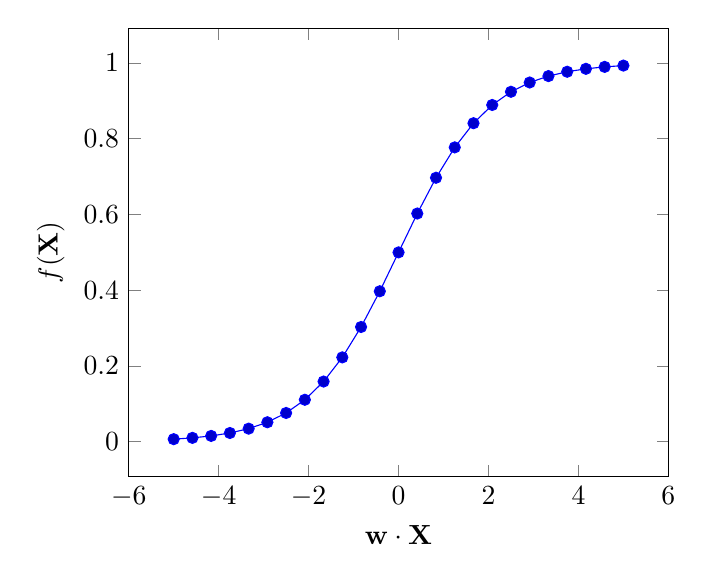
\begin{tikzpicture}
	\begin{axis}[
		xlabel=$\weights\cdot\X$,
		ylabel=$f(\X)$
	]
\addplot {1/(1+ e^-x)}; \end{axis}
\end{tikzpicture}
\end{center}
\end{frame}

\begin{frame}{SGD results}
	With the right $\eta$ it did comparably well against previous methods, but nothing significantly better.\\\
	I also tried $\eta=5\cdot10^{-1}$ to $\eta=5\cdot10^{-4}$ but resulted in buffer overflow
	when calculating the exponent.
	\begin{center}
		\footnotesize
		\begin{tabular}{ | l | c | c | c | }
			\hline
		& $Pr_{error}$		  & $T$-score			   &	Visit/Post\\
			\hline
	$\eta=5\cdot10^{-5}$ &	    0.499 &	  1595.563 &	    19.097 \\
	$\eta=5\cdot10^{-6}$ &	    0.501 &	  1525.705 &	    19.122 \\
	$\eta=5\cdot10^{-7}$ &	    0.502 &	  1440.440 &	    19.121 \\
			\rowcolor{green}
	$\eta=5\cdot10^{-8}$ &	    0.501 &	  1407.172 &	    19.108 \\
	$\eta=5\cdot10^{-9}$ &	    0.502 &	  1416.182 &	    19.110 \\
	$\eta=5\cdot10^{-10}$ &	    0.501 &	  1451.729 &	    19.106 \\
	$\eta=5\cdot10^{-11}$ &	    0.501 &	  1482.868 &	    19.104 \\
	$\eta=5\cdot10^{-12}$ &	    0.501 &	  1487.555 &	    19.104 \\
			\hline
		\end{tabular}
	\end{center}

	Is there a name for this?
\end{frame}

\begin{frame}{Work in progress...}
	\large
	\begin{enumerate}
		\item Another (better) metric for prediction models.
		\item Better way to present $T$-scores and Post/Visit ratios.
		\item Types of discussion (topic modeling?) and relationships with time intervals
		\item Full-scale evaluation for entire forum
		\item More datasets!
	\end{enumerate}
\end{frame}
\end{document}
